\documentclass[14pt,a4paper]{article}

\usepackage[russian]{babel}
\usepackage{hyperref} % for hyperlinks
\usepackage{indentfirst}
\usepackage{float}
\usepackage{geometry}
\usepackage{graphicx}
\usepackage{verbatim}
\usepackage{longtable}
\usepackage{amssymb}

\setlength{\parindent}{0.5cm}
\geometry{top=2cm, bottom=2cm, left=1.5cm, right=1.5cm}
\renewcommand{\thesubsection}{\arabic{subsection}}

\newcommand{\customtitle}[2]{%
\begin{titlepage}
  \begin{center}
    {\large\scshape\bfseries
    МИНИСТЕРСТВО НАУКИ И ВЫСШЕГО ОБРАЗОВАНИЯ РОССИЙСКОЙ ФЕДЕРАЦИИ\\
    ФЕДЕРАЛЬНОЕ ГОСУДАРСТВЕННОЕ АВТОНОМНОЕ ОБРАЗОВАТЕЛЬНОЕ УЧРЕЖДЕНИЕ ВЫСШЕГО
    ОБРАЗОВАНИЯ\\
    «СЕВЕРО-КАВКАЗСКИЙ ФЕДЕРАЛЬНЫЙ УНИВЕРСИТЕТ»\\
    ФАКУЛЬТЕТ МАТЕМАТИКИ И КОМПЬЮТЕРНЫХ НАУК ИМЕНИ ПРОФЕССОРА Н.И.ЧЕРВЯКОВА}
    \vfill
    \Large{\textbf{ЛАБОРАТОРНАЯ РАБОТА №#1}}\\[2mm]
    \large{Алгоритмизация и программирование}\\[6mm]
    \large{\textbf{#2}}\\[20mm]
  \end{center}
  \begin{flushright}
    \large{
      \textbf{Выполнил студент:}\\
      Сивко Иван Андреевич\\
      студент 2 курса\\
      группа ПМИ-б-о-23-2,\\
      направление подготовки 01.03.02\\[5mm]
      \textbf{Проверил:}\\
      Ассистент кафедры вычислительной\\
      математики и кибернетики, к.ф.-м.н.,\\
      Черкашина Анастасия Андреевна}
  \end{flushright}
  \vfill
  \centerline{ \the\year\ г. }
\end{titlepage}
    }


\newenvironment{fancyblock}
  {\large\bfseries\scshape}
  {}

\begin{document}
\customtitle{19}{Множества}
\large{\textbf{
\centerline{Вариант 9}
Цель:
}}
\begin{small}
  \begin{itemize}
    \item Совершенствование навыков разработки программ в среде программирования MS Visual Studio
    \item Совершенствование навыков в программировании с использованием множеств
    \item Исследование процесса формирования множеств
    \item Исследование операций с элементами множеств
  \end{itemize}
\end{small}
\section*{Задание 1}
\subsection{Условие:}
Дан текст из строчных латинских букв, за которым следует точка. Вывести на
экран все буквы входящие в текст по одному разу.
\subsection{Алгоритм / Мат. модель}
Программа анализирует строку, состоящую из строчных латинских букв,
завершающуюся точкой, и выводит все уникальные символы этой строки, исключая
пробелы. Для этого используется структура данных, обеспечивающая хранение
уникальных элементов (в данном случае — множества). Алгоритм работает следующим
образом:
\begin{enumerate}
  \item \textbf{Чтение входных данных:}\\
    Программа сначала проверяет наличие аргументов командной строки. Если они
    есть, строка собирается из всех переданных аргументов. В противном случае
    программа запрашивает строку у пользователя через стандартный ввод,
    ограничивая ввод точкой, чтобы исключить символы после неё.
  \item \textbf{Использование множества для хранения уникальных символов:}\\
    Весь текст из строки помещается в стандартное множество \texttt{std::set},
    которое автоматически удаляет все дубликаты, оставляя только уникальные
    символы.
  \item \textbf{Фильтрация пробелов:}\\
    При выводе уникальных символов из множества проверяется, что символ не
    является пробелом. Это делается с помощью стандартной функции
    \texttt{isspace}.
  \item \textbf{Вывод результата:}\\
    Уникальные символы выводятся на экран через пробел.
  \item \textbf{Завершение работы программы:}\\
    После выполнения всех операций программа корректно завершает выполнение,
    возвращая код \texttt{EXIT\_SUCCESS}.
\end{enumerate}
\begin{table}[H]
  \centering
  \resizebox{\textwidth}{!}{
    \begin{tabular}{|l|l|p{8cm}|} \hline
      \textbf{Название} & \textbf{Тип} & \textbf{Описание} \\ \hline
      \multicolumn{3}{|l|}{\textbf{Переменные main}} \\ \hline
      inputStr & std::string & Строка, в которой будет храниться весь ввод пользователя или аргументы командной строки. \\ \hline
      chr & char & Переменная, которая используется для итерации по символам строки в процессе вывода уникальных символов. \\ \hline
    \end{tabular}
  }
  \caption{Переменные, функции и структуры, используемые в программе}
  \label{tabel:1}
\end{table}
\subsection{Диаграмма:}
\begin{figure}[H]
  \centering
  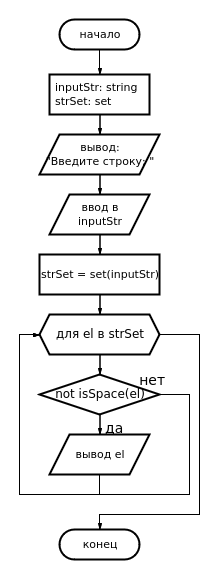
\includegraphics[height=0.4\textheight]{data/diagram19_1.png}
\end{figure}
\subsection{Код:}
\verbatiminput{data/task19_1.cpp}
\href{https://raw.githubusercontent.com/John1400800/stuff/refs/heads/main/c_learning/home_works/task19_1.cpp}{source code}
\subsection{Результат работы программы:}
\begin{figure}[H]
  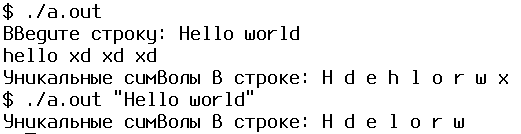
\includegraphics[width=0.5\textwidth]{data/demo19_1.png}
\end{figure}
\section*{Задание 2}
Выбрав произвольные множества А, В и С с ограничениями C++, проиллюстрировать
истинность следующих свойств операций над множествами и отношений между ними (с
нижним индексом в формулах используется дополнение множества до
соответствующего базового типа T, т.е. Bt = T – B, где B : set of T).
\setcounter{subsection}{0}
\subsection{Условие:}
Выбрав произвольные множества А, В и С с ограничениями C++, проиллюстрировать
истинность следующих свойств операций над множествами и отношений между ними (с
нижним индексом в формулах используется дополнение множества до
соответствующего базового типа T, т.е. Bt = T – B, где B : set of T).
\begin{figure}[H]
  \centering
  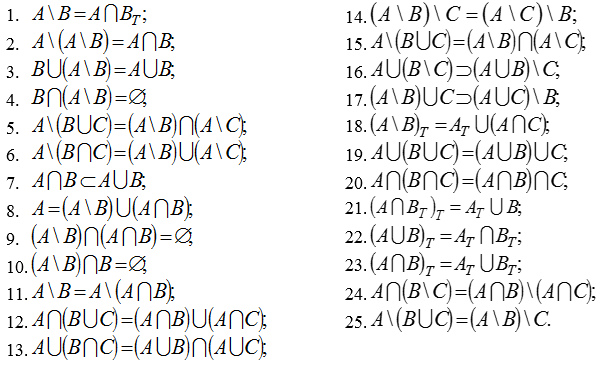
\includegraphics[width=0.7\textwidth]{data/condition19_2.png}
\end{figure}
\subsection{Алгоритм / Мат. модель}
Программа выполняет операции над двумя множествами целых чисел, введёнными пользователем. После ввода данных выполняются следующие шаги:
\begin{enumerate}
  \item \textbf{Инициализация переменных:}\\
    Программа инициализирует несколько переменных:
    \begin{itemize}
      \item \texttt{setA} и \texttt{setB} — множества типа \texttt{uint32\_t}, которые будут хранить элементы, введённые пользователем.
    \end{itemize}
  \item \textbf{Ввод данных:}
    \begin{itemize}
      \item Пользователь вводит элементы для множества \texttt{setA}. Ввод продолжается до тех пор, пока не будет введена пустая строка или некорректное значение.
      \item Ввод элементов множества \texttt{setB} аналогичен.
      \item Для каждого введённого числа функция \texttt{operator>>} пытается преобразовать строку в число и добавить его в соответствующее множество.
      \item Если ввод некорректен (например, введено нечисловое значение), программа выведет сообщение об ошибке и запросит ввод снова.
    \end{itemize}
  \item \textbf{Операции над множествами:}
    \begin{itemize}
      \item Программа выполняет операцию вычитания множества $A \setminus B$, используя перегруженный \texttt{operator-}. Результат выводится на экран.
      \item Затем выполняется операция пересечения множеств $A \cap B$ с использованием перегруженного \texttt{operator\&}. Результат также выводится на экран.
      \item Далее проверяется, является ли пересечение множества $A \setminus B$ и множества $A \cap B$ пустым с использованием операции \texttt{operator\&}. Результат выводится в виде логического значения \texttt{true} или \texttt{false}.
    \end{itemize}
  \item \textbf{Вывод результатов:}
    \begin{itemize}
      \item Программа выводит результат операции $A \setminus B$, затем результат операции $A \cap B$.
      \item В конце выводится результат проверки условия $(A \setminus B) \cap (A \cap B) = \varnothing$, которое возвращает логическое значение, подтверждающее или опровергающее пустоту пересечения.
    \end{itemize}
\end{enumerate}
\begin{table}[H]
  \centering
  \resizebox{\textwidth}{!}{
    \begin{tabular}{|l|l|p{8cm}|} \hline
      \textbf{Название} & \textbf{Тип} & \textbf{Описание} \\ \hline
      \multicolumn{3}{|l|}{\textbf{Функции}} \\ \hline
      operator>>() & std::istream\& & Перегрузка оператора ввода для ввода множества. Читает числа из потока и добавляет их в множество. \\ \hline
      operator<<() & std::ostream\& & Перегрузка оператора вывода для вывода множества в стандартный поток вывода. \\ \hline
      operator-() & std::set<T> & Перегрузка оператора вычитания для множеств, возвращающая элементы первого множества, которые не принадлежат второму. \\ \hline
      operator\&() & std::set<T> & Перегрузка оператора пересечения для множеств, возвращающая элементы, общие для двух множеств. \\ \hline
      \multicolumn{3}{|l|}{\textbf{Переменные main}} \\ \hline
      setA & std::set<uint32\_t> & Множество для хранения элементов первого множества, введенного пользователем. \\ \hline
      setB & std::set<uint32\_t> & Множество для хранения элементов второго множества, введенного пользователем. \\ \hline
    \end{tabular}
  }
  \caption{Переменные, функции и типы данных, используемые в программе}
  \label{tabel:1}
\end{table}
\subsection{Диаграмма:}
\begin{figure}[H]
  \centering
  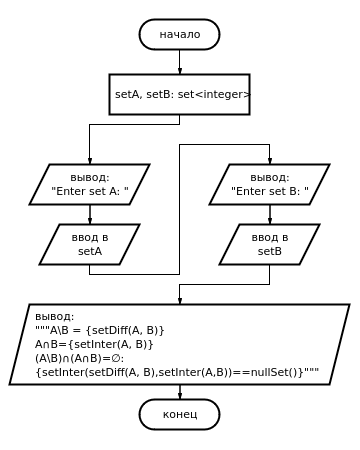
\includegraphics[height=0.4\textheight]{data/diagram19_2.png}
\end{figure}
\subsection{Код:}
\verbatiminput{data/task19_2.cpp}
\href{https://raw.githubusercontent.com/John1400800/stuff/refs/heads/main/c_learning/home_works/task19_2.cpp}{source code}
\subsection{Результат работы программы:}
\begin{figure}[H]
  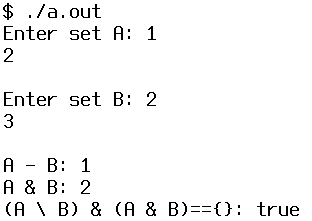
\includegraphics[width=0.3\textwidth]{data/demo19_2.png}
\end{figure}
\end{document}


